%=================================================================
% CSE 4345 — Big Data Analytics
% Week 10, Part 2: Seminal Research & Case Study
% Department of CSE, Premier University
%
% SEMINAL PAPERS:
%   Kwak et al. (2010) — What is Twitter, a Social Network or a
%   News Media? WWW 2010. (cited >7,000 times)
%
%   Taylor & Letham (2018) — Forecasting at Scale (Prophet).
%   The American Statistician 72(1). (cited >1,500 times)
%
% CASE STUDY:
%   CDC BioSense & Flu Surveillance (2009–2022): syndromic
%   surveillance at national scale; Prophet-based nowcasting
%   of influenza burden; lessons from Google Flu Trends failure
%=================================================================

\documentclass[aspectratio=169,10pt]{beamer}

%---------- Packages ----------
\usepackage[utf8]{inputenc}
\usepackage[T1]{fontenc}
\usepackage{booktabs}
\usepackage{xcolor}
\usepackage{tikz}
\usetikzlibrary{shapes.geometric, positioning, arrows.meta,
                decorations.pathreplacing}
\usepackage{amsmath}
\usepackage{graphicx}
\usepackage{multicol}
\usepackage{enumerate}
\usepackage{array}

%---------- Theme ----------
\usetheme{Madrid}

%---------- Premier University Color Identity ----------
\definecolor{PUNavy}{RGB}{10,36,99}
\definecolor{PUGold}{RGB}{197,151,37}
\definecolor{PULightBlue}{RGB}{210,228,255}
\definecolor{PUTeal}{RGB}{0,100,100}
\definecolor{PUGray}{RGB}{90,90,90}
\definecolor{PURed}{RGB}{160,30,30}
\definecolor{PUGreen}{RGB}{30,120,60}
\definecolor{PUPurple}{RGB}{90,30,120}
\definecolor{PUOrange}{RGB}{190,90,20}

\setbeamercolor{palette primary}{bg=PUNavy, fg=white}
\setbeamercolor{palette secondary}{bg=PUNavy!85, fg=white}
\setbeamercolor{palette tertiary}{bg=PUNavy!70, fg=white}
\setbeamercolor{palette quaternary}{bg=PUNavy, fg=white}
\setbeamercolor{structure}{fg=PUNavy}
\setbeamercolor{title}{bg=PUNavy, fg=PUGold}
\setbeamercolor{subtitle}{fg=white}
\setbeamercolor{frametitle}{bg=PUNavy, fg=PUGold}
\setbeamercolor{alerted text}{fg=PUGold!85!black}
\setbeamercolor{block title}{bg=PUNavy, fg=white}
\setbeamercolor{block body}{bg=PULightBlue!45}
\setbeamercolor{block title alerted}{bg=PUGold!80!black, fg=white}
\setbeamercolor{block body alerted}{bg=PUGold!12}
\setbeamercolor{block title example}{bg=PUTeal, fg=white}
\setbeamercolor{block body example}{bg=PUTeal!10}
\setbeamercolor{section in toc}{fg=PUNavy}
\setbeamercolor{itemize item}{fg=PUGold!80!black}
\setbeamercolor{itemize subitem}{fg=PUNavy!70}

\setbeamertemplate{navigation symbols}{}
\setbeamertemplate{itemize item}{\scriptsize\raise1.5pt\hbox{\textbullet}}
\setbeamertemplate{itemize subitem}{\scriptsize\raise1pt\hbox{--}}

%---------- Section separator ----------
\AtBeginSection[]{
  \begin{frame}[plain]
    \vfill
    \centering
    \begin{beamercolorbox}[sep=12pt,center,shadow=true,rounded=true]{block title}
      \usebeamerfont{title}\insertsectionhead\par
    \end{beamercolorbox}
    \vfill
  \end{frame}
}

%---------- Helper: citation box ----------
\newenvironment{paperbox}[1]{%
  \setbeamercolor{block title}{bg=PUNavy!90,fg=PUGold}
  \setbeamercolor{block body}{bg=PUNavy!6}
  \begin{block}{#1}}{%
  \end{block}}

%---------- Custom footline ----------
\setbeamertemplate{footline}{
  \leavevmode\hbox{%
    \begin{beamercolorbox}[wd=.333\paperwidth,ht=2.25ex,dp=1ex,center]{palette primary}
      \usebeamerfont{author in head/foot}\insertshortauthor
    \end{beamercolorbox}%
    \begin{beamercolorbox}[wd=.334\paperwidth,ht=2.25ex,dp=1ex,center]{palette secondary}
      \usebeamerfont{title in head/foot}\insertshorttitle
    \end{beamercolorbox}%
    \begin{beamercolorbox}[wd=.333\paperwidth,ht=2.25ex,dp=1ex,right]{palette primary}
      \usebeamerfont{date in head/foot}
      \insertframenumber{} / \inserttotalframenumber\hspace*{2ex}
    \end{beamercolorbox}}%
  \vskip0pt%
}

%---------- Title metadata ----------
\title[CSE 4345 \textbar{} Week 10, Part 2]{CSE 4345: Big Data Analytics}
\subtitle{Week 10, Part 2 \textemdash\ Seminal Research \& Case Study}
\author[Dept.\ of CSE]{Department of Computer Science \& Engineering\\[4pt]
       \small Premier University, Chittagong}
\institute{}
\date{Semester 2026}

%=================================================================
\begin{document}
%=================================================================

\begin{frame}
  \titlepage
\end{frame}

%----------------------------------------------------------------
\begin{frame}{Part 2 Overview — Week 10}
  \begin{columns}[T]
    \column{0.47\textwidth}
      \begin{block}{Today's Agenda}
        \tableofcontents
      \end{block}
    \column{0.50\textwidth}
      \begin{exampleblock}{Seminal Papers Covered}
        \begin{enumerate}
          \item Kwak, H., Lee, C., Park, H., \& Moon, S. (2010).
                \textit{What is Twitter, a Social Network or a
                News Media?} ACM WWW 2010.
          \item Taylor, S.~J., \& Letham, B. (2018).
                \textit{Forecasting at Scale.}
                \textit{The American Statistician, 72}(1).
        \end{enumerate}
      \end{exampleblock}
      \vspace{6pt}
      \begin{alertblock}{Case Study}
        CDC BioSense \& ILINet Flu Surveillance (2009--2022):
        syndromic surveillance of \textbf{3{,}500+ hospitals},
        Prophet-based flu nowcasting, and the cautionary tale
        of \textbf{Google Flu Trends} (2008--2015).
      \end{alertblock}
      \vspace{4pt}
      \begin{block}{CLO Addressed}
        \textbf{CLO4} — Solve problems using social media,
        time-series, and health data analytics\\
        \textbf{PLO(c,d)}
      \end{block}
  \end{columns}
\end{frame}

%================================================================
\section{Paper 1 — Kwak et al.\ (2010): Twitter Network Analysis}
%================================================================

%----------------------------------------------------------------
\begin{frame}{Research Landscape: Social Network Analysis}
  \begin{center}
  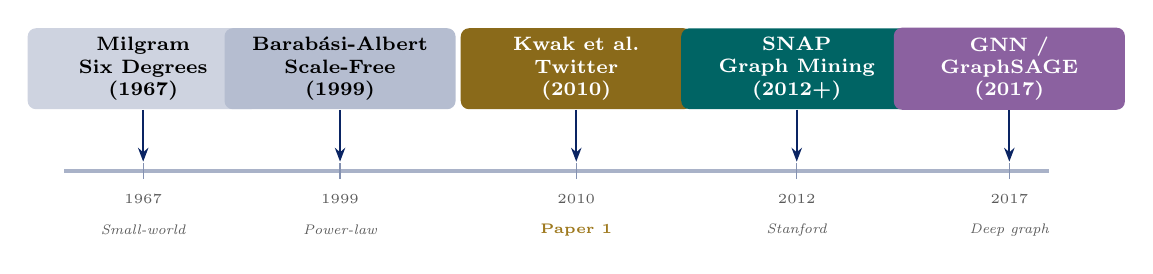
\begin{tikzpicture}[
      nbox/.style={rectangle, rounded corners=3pt, minimum width=2.9cm,
                   minimum height=0.9cm, text width=2.7cm, align=center,
                   font=\scriptsize\bfseries},
      arr/.style={-{Stealth[length=5pt]}, draw=PUNavy, thick}
    ]
    \draw[PUNavy!35, very thick] (0,0) -- (12.5,0);

    \node[nbox, fill=PUNavy!20]              (milg) at (1.0, 1.3)
          {Milgram\\Six Degrees\\(1967)};
    \node[nbox, fill=PUNavy!30]              (ba)   at (3.5, 1.3)
          {Barab{\'a}si-Albert\\Scale-Free\\(1999)};
    \node[nbox, fill=PUGold!70!black, text=white] (kwak) at (6.5, 1.3)
          {Kwak et al.\\Twitter\\(2010)};
    \node[nbox, fill=PUTeal, text=white]     (snap) at (9.3, 1.3)
          {SNAP\\Graph Mining\\(2012+)};
    \node[nbox, fill=PUPurple!70, text=white](gnn)  at (12.0,1.3)
          {GNN /\\GraphSAGE\\(2017)};

    \foreach \x/\y in {1.0/1967, 3.5/1999, 6.5/2010, 9.3/2012, 12.0/2017}{
      \draw[PUNavy!50] (\x,0.1) -- (\x,-0.1);
      \node[font=\tiny, text=PUGray] at (\x,-0.35) {\y};
    }

    \draw[arr] (milg)--(1.0, 0.12);
    \draw[arr] (ba)  --(3.5, 0.12);
    \draw[arr] (kwak)--(6.5, 0.12);
    \draw[arr] (snap)--(9.3, 0.12);
    \draw[arr] (gnn) --(12.0,0.12);

    \node[font=\tiny\itshape, text=PUGray]           at (1.0, -0.75) {Small-world};
    \node[font=\tiny\itshape, text=PUGray]           at (3.5, -0.75) {Power-law};
    \node[font=\tiny\bfseries, text=PUGold!80!black] at (6.5, -0.75) {Paper 1};
    \node[font=\tiny\itshape, text=PUGray]           at (9.3, -0.75) {Stanford};
    \node[font=\tiny\itshape, text=PUGray]           at (12.0,-0.75) {Deep graph};
  \end{tikzpicture}
  \end{center}
  \vspace{4pt}
  \begin{alertblock}{Why This Paper Matters for Big Data}
    Twitter's 2010 graph had \textbf{41.7 million users} and
    \textbf{1.47 billion directed following edges}.
    Crawling, storing, and analysing it required HDFS + MapReduce
    — the paper is one of the first empirical social network studies
    at Big Data scale.
    Its findings shaped every subsequent social media analytics
    platform, from Twitter's own Trends algorithm to CDC's
    infodemic surveillance.
  \end{alertblock}
\end{frame}

%----------------------------------------------------------------
\begin{frame}{Kwak et al.\ (2010): Publication Context}
  \begin{columns}[T]
    \column{0.53\textwidth}
      \begin{paperbox}{Full Citation}
        Kwak, H., Lee, C., Park, H., \& Moon, S. (2010).
        \textbf{What is Twitter, a Social Network or a News Media?}
        In \textit{Proceedings of the 19th International
        Conference on the World Wide Web (WWW '10)},
        pp.~591--600. Raleigh, NC, USA. ACM.\\[5pt]
        \textbf{Venue:} ACM WWW — Rank A* (CORE), top Web venue\\
        \textbf{Cited by:} $>$7{,}000 (Google Scholar, 2024)\\
        \textbf{Authors:} Haewoon Kwak, Changhyun Lee, Hosung Park,
        Sue Moon — KAIST (Korea Advanced Institute of Science
        and Technology)
      \end{paperbox}
      \vspace{5pt}
      \begin{exampleblock}{The Central Question}
        \begin{center}
        \large\color{PUNavy}
        \textit{Is Twitter a social network
        (mutual relationships, like Facebook)
        or a news medium
        (one-to-many broadcasting)?}
        \end{center}
        \vspace{4pt}
        \small The answer has profound implications for recommendation
        algorithms, misinformation spread, and public health surveillance.
      \end{exampleblock}

    \column{0.44\textwidth}
      \begin{block}{Dataset}
        \renewcommand{\arraystretch}{1.25}
        \begin{tabular}{@{}ll@{}}
          \toprule
          \textbf{Metric} & \textbf{Value} \\
          \midrule
          Users crawled          & 41.7 million \\
          Following edges        & 1.47 billion \\
          Tweets collected       & 106 million \\
          Crawl duration         & June 2009 \\
          Crawl method           & BFS via Twitter API \\
          Storage                & HDFS cluster \\
          Analysis               & MapReduce (Hadoop) \\
          \bottomrule
        \end{tabular}
      \end{block}
      \vspace{5pt}
      \begin{alertblock}{Infrastructure Note}
        Collecting 1.47 billion edges required rate-limit-aware
        BFS crawling over 3 weeks, producing $\approx$40~GB
        of compressed adjacency data — one of the first
        Big Data social graph studies.
      \end{alertblock}
  \end{columns}
\end{frame}

%----------------------------------------------------------------
\begin{frame}{Technical Contribution 1 — Network Topology Findings}
  \begin{columns}[T]
    \column{0.50\textwidth}
      \begin{block}{Key Structural Results}
        \begin{enumerate}
          \item \textbf{Highly asymmetric}: 77.9\% of users
                have a follower who does not follow them back.
                Compare to Facebook (mutual friendship required):
                Twitter is a \emph{directed} graph, not undirected.
          \item \textbf{Power-law degree distribution}: follower
                counts follow $P(k) \propto k^{-\alpha}$ with
                $\alpha \approx 2.276$ for in-degree (followers).
                The top 0.05\% of users (celebrities) have
                $>$1 million followers.
          \item \textbf{Small world}: average shortest path
                length = \textbf{4.12 hops} across 41.7M users —
                slightly less than Milgram's ``six degrees.''
          \item \textbf{Reciprocity rate}: only 22.1\% of
                following relationships are mutual — far lower
                than Facebook ($\approx$100\%).
        \end{enumerate}
      \end{block}
      \vspace{4pt}
      \begin{exampleblock}{PageRank vs.\ Follower Count}
        The paper's most cited finding: users ranked by
        \textbf{PageRank} (influence in the directed graph)
        differ substantially from those ranked by raw
        \textbf{follower count}.
        A user with 1M followers who is followed \emph{by}
        many high-PageRank users outranks a celebrity with
        5M low-influence followers.
      \end{exampleblock}

    \column{0.47\textwidth}
      \begin{center}
      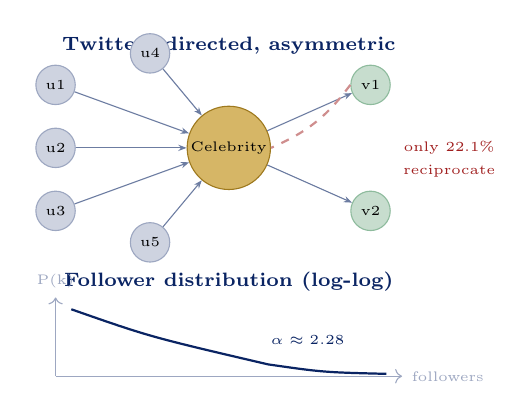
\begin{tikzpicture}[
          nd/.style={circle, minimum size=0.5cm, font=\tiny,
                     inner sep=1pt},
          arr/.style={-{Stealth[length=3pt]}, draw=PUNavy!60, thin}
        ]
        \node[font=\scriptsize\bfseries, text=PUNavy] at (0, 4.3)
              {Twitter: directed, asymmetric};

        % Celebrity node
        \node[nd, fill=PUGold!70, draw=PUGold!80!black, minimum size=1.0cm]
              (cel) at (0, 3.0) {\tiny Celebrity};
        % Many followers pointing in
        \node[nd, fill=PUNavy!20, draw=PUNavy!40] (f1) at (-2.2, 3.8) {u1};
        \node[nd, fill=PUNavy!20, draw=PUNavy!40] (f2) at (-2.2, 3.0) {u2};
        \node[nd, fill=PUNavy!20, draw=PUNavy!40] (f3) at (-2.2, 2.2) {u3};
        \node[nd, fill=PUNavy!20, draw=PUNavy!40] (f4) at (-1.0, 4.2) {u4};
        \node[nd, fill=PUNavy!20, draw=PUNavy!40] (f5) at (-1.0, 1.8) {u5};

        \draw[arr] (f1)--(cel); \draw[arr] (f2)--(cel);
        \draw[arr] (f3)--(cel); \draw[arr] (f4)--(cel);
        \draw[arr] (f5)--(cel);

        % Celebrity broadcasts out (but not mutual)
        \node[nd, fill=PUGreen!25, draw=PUGreen!50] (n1) at (1.8, 3.8) {v1};
        \node[nd, fill=PUGreen!25, draw=PUGreen!50] (n2) at (1.8, 2.2) {v2};
        \draw[arr] (cel)--(n1); \draw[arr] (cel)--(n2);

        % Reciprocity annotation
        \draw[PURed!50, dashed, thick] (n1.west) to[bend left=15] (cel.east);
        \node[font=\tiny, text=PURed] at (2.8, 3.0) {only 22.1\%};
        \node[font=\tiny, text=PURed] at (2.8, 2.7) {reciprocate};

        % Power-law mini chart
        \node[font=\scriptsize\bfseries, text=PUNavy] at (0, 1.3)
              {Follower distribution (log-log)};
        \draw[PUNavy!40, ->] (-2.2, 0.1) -- (2.2, 0.1)
              node[right, font=\tiny] {followers};
        \draw[PUNavy!40, ->] (-2.2, 0.1) -- (-2.2, 1.1)
              node[above, font=\tiny] {P(k)};
        \draw[PUNavy, thick]
              (-2.0,0.95) .. controls (-1.0,0.6) .. (0.5,0.25)
              .. controls (1.2,0.15) .. (2.0,0.13);
        \node[font=\tiny, text=PUNavy] at (1.0, 0.55)
              {$\alpha\approx 2.28$};
      \end{tikzpicture}
      \end{center}
  \end{columns}
\end{frame}

%----------------------------------------------------------------
\begin{frame}{Technical Contribution 2 — Twitter as News Medium}
  \begin{columns}[T]
    \column{0.50\textwidth}
      \begin{block}{Trending Topics: News, Not Social Chatter}
        Kwak et al.\ analysed 106M tweets to characterise
        \textbf{Trending Topics}:
        \begin{itemize}
          \item \textbf{85\%} of trending topics were \emph{headline
                news} (breaking news, political events, entertainment
                releases) — not personal conversations
          \item Only 15\% were social memes or conversational trends
          \item The median duration of a trending topic:
                \textbf{17.5 hours} — the lifespan of a news cycle
          \item A breaking news topic reaches \textbf{peak tweet rate}
                within \textbf{15 minutes} of the event
        \end{itemize}
        \textbf{Conclusion}: Twitter functions as a
        \textbf{real-time news wire}, not a social network.
        Its information diffusion speed rivals (and sometimes beats)
        professional news agencies.
      \end{block}
      \vspace{4pt}
      \begin{alertblock}{Information Cascade Finding}
        Retweet cascades are \textbf{wide and shallow} (breadth $\gg$
        depth), unlike friendship cascades which are deep.
        A celebrity's tweet is retweeted widely in one hop;
        a friend's post travels through a long chain.
      \end{alertblock}

    \column{0.47\textwidth}
      \begin{block}{Impact on Public Health Surveillance}
        The Twitter-as-news-media finding directly enabled
        \textbf{social media epidemiology}:
        \begin{itemize}
          \item If Twitter reflects real-world events within minutes,
                flu-related tweets should correlate with actual
                flu incidence
          \item Culotta (2010) and Signorini et al.\ (2011) used
                Twitter keyword streams to estimate influenza rates
                \emph{two weeks ahead} of CDC official reports
          \item CDC now monitors \textbf{Twitter/X for infodemic signals}:
                vaccine misinformation, outbreak rumours,
                mental health crisis language
          \item The paper's directed-graph model of information flow
                is the basis of \textbf{contact tracing network models}
                used in COVID-19 policy
        \end{itemize}
      \end{block}
  \end{columns}
\end{frame}

%================================================================
\section{Paper 2 — Taylor \& Letham (2018): Prophet}
%================================================================

%----------------------------------------------------------------
\begin{frame}{Taylor \& Letham (2018): Publication Context \& Model}
  \begin{columns}[T]
    \column{0.53\textwidth}
      \begin{paperbox}{Full Citation}
        Taylor, S.~J., \& Letham, B. (2018).
        \textbf{Forecasting at Scale.}
        \textit{The American Statistician, 72}(1), 37--45.
        (First published online 2017.)\\[5pt]
        \textbf{Venue:} The American Statistician (ASA, peer-reviewed)\\
        \textbf{Cited by:} $>$1{,}500 (Google Scholar, 2024)\\
        \textbf{Authors:} Sean J.\ Taylor \& Benjamin Letham
        (Facebook Core Data Science team)\\[4pt]
        \textbf{Code:} Apache-licensed at
        \texttt{github.com/facebook/prophet};
        available for Python and R
      \end{paperbox}
      \vspace{5pt}
      \begin{block}{The Decomposable Model}
        \[
          y(t) = g(t) + s(t) + h(t) + \varepsilon_t
        \]
        \begin{itemize}
          \item $g(t)$: \textbf{trend} (piecewise linear or logistic)
          \item $s(t)$: \textbf{seasonality} (Fourier series)
          \item $h(t)$: \textbf{holiday effects} (configurable list)
          \item $\varepsilon_t$: noise (Gaussian)
        \end{itemize}
        Parameters estimated via \textbf{Stan} (Bayesian MAP).
      \end{block}

    \column{0.44\textwidth}
      \begin{center}
      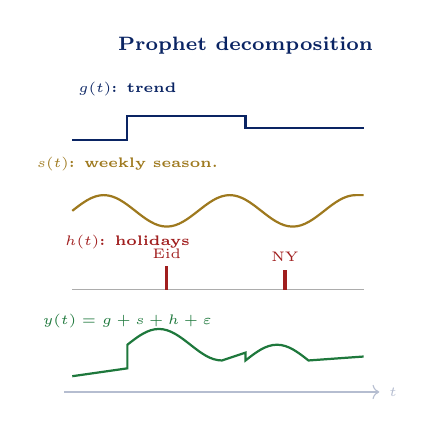
\begin{tikzpicture}[
          arr/.style={-{Stealth[length=4pt]}, draw=PUNavy, thick}
        ]
        \node[font=\scriptsize\bfseries, text=PUNavy] at (0, 4.6)
              {Prophet decomposition};

        % Trend
        \node[font=\tiny\bfseries, text=PUNavy] at (-1.5, 4.05) {$g(t)$: trend};
        \draw[PUNavy, thick]
              (-2.2,3.4) -- (-1.5,3.4) -- (-1.5,3.7)
              -- (0.0,3.7) -- (0.0,3.55) -- (1.5,3.55);

        % Seasonality
        \node[font=\tiny\bfseries, text=PUGold!80!black] at (-1.5,3.1)
              {$s(t)$: weekly season.};
        \draw[PUGold!80!black, thick]
              (-2.2,2.5) sin (-1.8,2.7) cos (-1.4,2.5)
              sin (-1.0,2.3) cos (-0.6,2.5)
              sin (-0.2,2.7) cos (0.2,2.5)
              sin (0.6,2.3) cos (1.0,2.5)
              sin (1.4,2.7) -- (1.5,2.7);

        % Holidays
        \node[font=\tiny\bfseries, text=PURed] at (-1.5,2.1)
              {$h(t)$: holidays};
        \draw[PUGray!50, thin] (-2.2,1.5)--(1.5,1.5);
        \draw[PURed, very thick] (-1.0,1.5) -- (-1.0,1.8);
        \draw[PURed, very thick] (0.5,1.5)  -- (0.5,1.75);
        \node[font=\tiny, text=PURed] at (-1.0,1.95) {Eid};
        \node[font=\tiny, text=PURed] at (0.5,1.92)  {NY};

        % Combined
        \node[font=\tiny\bfseries, text=PUGreen] at (-1.5,1.1)
              {$y(t) = g+s+h+\varepsilon$};
        \draw[PUGreen, thick]
              (-2.2,0.4) -- (-1.5,0.5) -- (-1.5,0.8)
              sin (-1.1,1.0) cos (-0.7,0.8)
              sin (-0.3,0.6) -- (0.0,0.7)
              -- (0.0,0.6) sin (0.4,0.8)
              cos (0.8,0.6) -- (1.5,0.65);

        % Axis
        \draw[PUNavy!30, ->] (-2.3,0.2)--(1.7,0.2)
              node[right,font=\tiny] {$t$};
      \end{tikzpicture}
      \end{center}
  \end{columns}
\end{frame}

%----------------------------------------------------------------
\begin{frame}{Prophet: Changepoints, Seasonality \& Scale}
  \begin{columns}[T]
    \column{0.50\textwidth}
      \begin{block}{Automatic Changepoint Detection}
        The trend $g(t)$ is \textbf{piecewise linear}:
        \[
          g(t) = (k + \mathbf{a}(t)^{\top}\boldsymbol{\delta})\,t
                 + (m + \mathbf{a}(t)^{\top}\boldsymbol{\gamma})
        \]
        where $\boldsymbol{\delta}$ are slope adjustments at
        automatically detected \textbf{changepoints}
        (structural breaks in trend).\\[5pt]
        \textbf{Sparse prior} on $\boldsymbol{\delta}$:
        most changepoints have $\delta_j \approx 0$;
        a few are large.
        This avoids overfitting while capturing genuine trend shifts.\\[5pt]
        \textbf{Fourier seasonality}:
        \[
          s(t) = \sum_{n=1}^{N}
          \left(a_n \cos\!\tfrac{2\pi n t}{P}
              + b_n \sin\!\tfrac{2\pi n t}{P}\right)
        \]
        $P = 365.25$ (annual), $P = 7$ (weekly);
        $N$ controls smoothness.
      \end{block}

    \column{0.47\textwidth}
      \begin{block}{Designed for Analysts, Not Statisticians}
        Prophet's key design goal was \textbf{scalable human-in-the-loop
        forecasting} at Facebook:
        \begin{itemize}
          \item Facebook needed forecasts for \textbf{thousands of
                business metrics} (DAU, ad impressions, revenue)
                updated daily
          \item Domain analysts (not statisticians) needed to
                \textbf{tune} forecasts — add known holidays,
                adjust trend flexibility, handle outliers
          \item \textbf{Interpretable parameters}: analysts understand
                ``weekly seasonality'' and ``holiday dip'' without
                understanding ARIMA lag orders
          \item \textbf{Robust to missing data and outliers}:
                the additive structure absorbs spikes without
                corrupting the trend estimate
        \end{itemize}
      \end{block}
      \vspace{4pt}
      \begin{alertblock}{Big Data Application}
        Facebook ran Prophet on \textbf{500{,}000+ time series}
        simultaneously using Spark's \texttt{applyInPandas} —
        one Prophet model per group (per country, per product,
        per cohort) executed in parallel across a cluster.
      \end{alertblock}
  \end{columns}
\end{frame}

%----------------------------------------------------------------
\begin{frame}{Impact Today — Kwak (2010) \& Taylor/Letham (2018)}
  \begin{columns}[T]
    \column{0.50\textwidth}
      \begin{block}{Kwak et al.\ — Downstream Impact}
        \begin{itemize}
          \item \textbf{Twitter Trending Topics algorithm}: the paper's
                finding that trending topics are news-driven shaped
                Twitter's later algorithm redesigns
          \item \textbf{Social media epidemiology}: CDC, WHO, and
                academic groups built flu, COVID, and mental health
                surveillance on the Twitter graph model
          \item \textbf{Fake news research}: the directed-cascade
                model of retweets is the reference network structure
                for misinformation propagation studies (Vosoughi 2018)
          \item \textbf{Influence maximisation} (Kempe et al.\ 2003
                + Kwak findings): seeding a campaign at
                high-PageRank nodes vs.\ high-follower nodes yields
                measurably different virality
        \end{itemize}
      \end{block}

    \column{0.47\textwidth}
      \begin{block}{Prophet — Downstream Impact}
        \begin{itemize}
          \item \textbf{Industry standard for business forecasting}:
                adopted by Airbnb, Uber, Walmart, and dozens of
                unicorn-stage startups for demand and revenue forecasting
          \item \textbf{Healthcare}: hospital admissions forecasting;
                ICU capacity planning during COVID-19 waves
          \item \textbf{Energy sector}: electricity demand
                forecasting with Prophet + temperature covariates
          \item \textbf{Spark vectorisation}: the \texttt{applyInPandas}
                + Prophet pattern (Week 10, Part 1) is now a
                canonical PySpark design pattern in production
          \item \textbf{NeuralProphet} (2021): replaces Fourier
                seasonality with neural networks; extends Prophet
                for complex, non-linear seasonality
        \end{itemize}
      \end{block}
  \end{columns}
\end{frame}

%================================================================
\section{Case Study — CDC Flu Surveillance \& the Google Flu Lesson}
%================================================================

%----------------------------------------------------------------
\begin{frame}{CDC Disease Surveillance Infrastructure}
  \begin{columns}[T]
    \column{0.52\textwidth}
      \begin{block}{The CDC ILINet and BioSense Systems}
        \textbf{ILINet} (Influenza-Like Illness Surveillance Network):
        \begin{itemize}
          \item $>$3{,}000 sentinel physicians in all 50 US states
                report weekly counts of ILI patients
                (\textit{fever + cough or sore throat})
          \item Data flows: clinic $\to$ state health dept $\to$
                CDC weekly report
          \item \textbf{Lag}: 1--2 weeks behind real time
          \item Used to issue \textbf{flu season start/end} and
                estimate excess mortality
        \end{itemize}
        \textbf{BioSense Platform}:
        \begin{itemize}
          \item Real-time electronic health data from
                \textbf{3{,}500+ emergency departments}
          \item Syndromes (flu-like, gastrointestinal, neurological)
                automatically extracted from visit chief complaints
          \item Near-real-time ($<$72 hr lag): enables
                \textbf{outbreak detection} before ILINet
        \end{itemize}
      \end{block}

    \column{0.45\textwidth}
      \begin{center}
      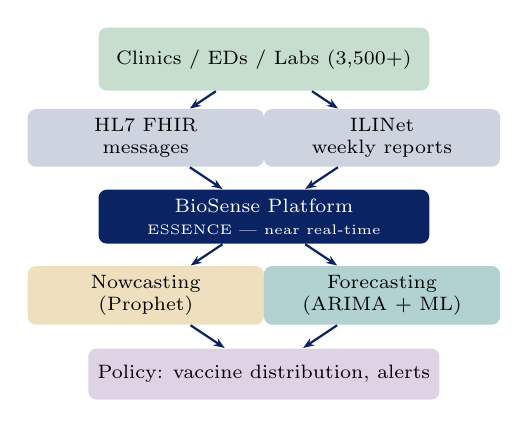
\begin{tikzpicture}[
          cb/.style={rectangle, rounded corners=3pt, minimum width=3.0cm,
                     minimum height=0.65cm, align=center, font=\scriptsize},
          arr/.style={-{Stealth[length=4pt]}, draw=PUNavy, thick}
        ]
        \node[cb, fill=PUGreen!25, minimum width=4.2cm,
              minimum height=0.8cm]
              (src) at (0, 4.5)
              {Clinics / EDs / Labs (3,500+)};

        \node[cb, fill=PUNavy!20] (hl7)  at (-1.5, 3.5)
              {HL7 FHIR\\messages};
        \node[cb, fill=PUNavy!20] (ili)  at (1.5,  3.5)
              {ILINet\\weekly reports};

        \node[cb, fill=PUNavy, text=white, minimum width=4.2cm]
              (bio)  at (0, 2.5)
              {BioSense Platform\\{\tiny ESSENCE — near real-time}};

        \node[cb, fill=PUGold!30] (now)  at (-1.5, 1.5)
              {Nowcasting\\(Prophet)};
        \node[cb, fill=PUTeal!30] (fore) at (1.5,  1.5)
              {Forecasting\\(ARIMA + ML)};

        \node[cb, fill=PUPurple!20, minimum width=4.2cm]
              (pol) at (0, 0.5)
              {Policy: vaccine distribution, alerts};

        \draw[arr] (src)  -- (hl7);
        \draw[arr] (src)  -- (ili);
        \draw[arr] (hl7)  -- (bio);
        \draw[arr] (ili)  -- (bio);
        \draw[arr] (bio)  -- (now);
        \draw[arr] (bio)  -- (fore);
        \draw[arr] (now)  -- (pol);
        \draw[arr] (fore) -- (pol);
      \end{tikzpicture}
      \end{center}
  \end{columns}
\end{frame}

%----------------------------------------------------------------
\begin{frame}{Google Flu Trends: A Big Data Cautionary Tale}
  \begin{columns}[T]
    \column{0.52\textwidth}
      \begin{block}{The Promise (2008--2011)}
        Google Flu Trends (GFT), launched 2008 (Ginsberg et al.,
        \textit{Nature} 2009):
        \begin{itemize}
          \item Correlated 45 flu-related search queries with
                ILINet data to \textbf{predict flu incidence}
                \emph{two weeks before} CDC official reports
          \item Initial accuracy: $r^2 = 0.97$ on 2003--2008 data
          \item Cited as the canonical example of
                \textbf{Big Data surpassing traditional surveillance}
        \end{itemize}
      \end{block}
      \vspace{5pt}
      \begin{alertblock}{The Failure (2012--2015)}
        GFT over-predicted flu rates by \textbf{$2\times$} in the
        2012--2013 season.
        Lazer et al.\ (\textit{Science} 2014) diagnosed three causes:
        \begin{enumerate}
          \item \textbf{Big Data hubris}: $r^2 = 0.97$ on 5 years
                of training data does not imply generalisation
          \item \textbf{Algorithm confounding}: Google's autocomplete
                algorithm changed query suggestions, altering
                the search feature distribution
          \item \textbf{Media amplification}: flu news coverage
                drove flu-related searches even when incidence
                was low, creating a \textbf{spurious correlation}
        \end{enumerate}
      \end{alertblock}

    \column{0.45\textwidth}
      \begin{block}{Prophet-Based Nowcasting: A Better Approach}
        Post-GFT failure, CDC and academic groups rebuilt
        flu forecasting using \textbf{Prophet + BioSense}:
        \begin{itemize}
          \item \textbf{BioSense ED visits} as the primary signal
                (direct medical observation, not proxy search data)
          \item \textbf{Prophet} models weekly and annual seasonality;
                detects changepoints at flu season start
          \item \textbf{Twitter signals} (Kwak paper) added as
                an \emph{exogenous covariate}, not a replacement
                for surveillance data
          \item \textbf{Ensemble}: CDC FluSight challenge (2013--present)
                combines Prophet, ARIMA, LSTM, and human
                expert forecasts — no single model wins every season
        \end{itemize}
      \end{block}
      \vspace{4pt}
      \begin{exampleblock}{Scale (2019--2020 season)}
        BioSense processed \textbf{38 million ED visits};
        Prophet models ran on 60 HHS regions simultaneously
        via Spark \texttt{applyInPandas}.
      \end{exampleblock}
  \end{columns}
\end{frame}

%----------------------------------------------------------------
\begin{frame}{Lessons Learned \& Discussion Questions}
  \begin{columns}[T]
    \column{0.52\textwidth}
      \begin{block}{Key Lessons from the CDC/GFT Case}
        \begin{enumerate}
          \item \textbf{Proxy data amplifies noise}:
                search queries capture \emph{health anxiety},
                not health incidence; proxy signals need
                causal validation before policy use
          \item \textbf{Algorithm transparency is a public health issue}:
                GFT failed because Google's internal autocomplete
                changes (opaque to CDC) shifted the feature distribution
          \item \textbf{Decomposability improves trust}:
                Prophet's $g + s + h$ structure lets epidemiologists
                inspect each component — unlike black-box deep
                learning forecasters
          \item \textbf{Ensemble beats any single model}:
                CDC FluSight's top performers (2013--2022) are
                always ensemble methods; Prophet is a strong component,
                not a standalone solution
          \item \textbf{Twitter adds lead time, not accuracy}:
                social media signals are available 2 weeks earlier
                than ILINet but with 30\% higher error;
                the trade-off is latency vs.\ precision
        \end{enumerate}
      \end{block}

    \column{0.45\textwidth}
      \begin{alertblock}{Discussion Questions \textmd{\tiny (CLO4)}}
        \begin{enumerate}
          \item Kwak et al.\ found Twitter's average shortest path
                is 4.12 hops over 41.7M users.
                If a misinformation tweet is retweeted by
                a high-PageRank account, estimate how many users
                it reaches within \textbf{3 hops} assuming
                an average out-degree of 45.
                What graph property makes this estimate an
                \textbf{overestimate}?
                \textit{[CLO4 — Apply]}
          \item A Prophet model for weekly hospital admissions
                has strong annual and weekly seasonality but
                misses a sudden COVID-19 wave onset.
                Identify which Prophet component should detect
                this changepoint and explain what prior
                hyperparameter controls the model's sensitivity
                to new changepoints.
                \textit{[CLO4 — Analyse]}
          \item Design a \textbf{dengue fever surveillance system}
                for Bangladesh using BioSense-style ED data,
                Twitter signals, and Prophet forecasting.
                Specify: data sources, pipeline architecture
                (Kafka + Spark), model inputs, and how you
                would validate the system before policy use.
                \textit{[CLO4 — Design]}
        \end{enumerate}
      \end{alertblock}
  \end{columns}
\end{frame}

%================================================================
\section{Live Exercise}
%================================================================

%----------------------------------------------------------------
\begin{frame}[fragile]{Live Exercise — Prophet Flu Forecasting in Python}
  \begin{columns}[T]
    \column{0.50\textwidth}
      \begin{block}{Task (25 minutes, pairs)}
        Fit a \textbf{Prophet} model to synthetic weekly flu
        incidence data and produce a 12-week forecast.\\[5pt]
        \textbf{Goals}:
        \begin{enumerate}\setlength\itemsep{1pt}
          \item Generate 3 years of synthetic weekly ILI data
                with annual seasonality + noise.
          \item Fit Prophet with yearly and weekly seasonality.
          \item Plot the forecast with 95\% uncertainty intervals.
          \item Add a \textbf{holiday} for ``Eid'' (spike in
                healthcare visits) and observe the effect.
          \item Change \texttt{changepoint\_prior\_scale}
                from 0.05 to 0.5 and compare trend flexibility.
        \end{enumerate}
      \end{block}
      \vspace{4pt}
      \begin{exampleblock}{Install}
        \scriptsize\texttt{pip install prophet matplotlib pandas}
      \end{exampleblock}

    \column{0.47\textwidth}
      \begin{exampleblock}{Python Skeleton}
        \scriptsize
        \begin{verbatim}
import pandas as pd
import numpy as np
from prophet import Prophet
import matplotlib.pyplot as plt

rng = np.random.default_rng(42)
dates = pd.date_range("2021-01-04",
                       periods=156, freq="W")
# Annual flu seasonality + noise
ili = (5 + 3*np.sin(
         2*np.pi*np.arange(156)/52
         - np.pi/2)
       + rng.normal(0, 0.5, 156)).clip(0)

df = pd.DataFrame({"ds": dates, "y": ili})

# Optional: add Eid holiday
holidays = pd.DataFrame({
  "holiday":  "Eid",
  "ds":       pd.to_datetime([
                "2021-05-13","2022-05-03",
                "2023-04-22"]),
  "lower_window": 0,
  "upper_window": 3,
})

m = Prophet(
  yearly_seasonality=True,
  weekly_seasonality=False,
  changepoint_prior_scale=0.05,
  holidays=holidays)
m.fit(df)

future   = m.make_future_dataframe(
             periods=12, freq="W")
forecast = m.predict(future)
m.plot(forecast)
m.plot_components(forecast)
plt.show()
        \end{verbatim}
      \end{exampleblock}
  \end{columns}
\end{frame}

%================================================================
\section*{References}
%================================================================

%----------------------------------------------------------------
\begin{frame}{References}
  \begin{block}{Seminal Papers}
    \begin{itemize}
      \item Kwak, H., Lee, C., Park, H., \& Moon, S. (2010).
            What is Twitter, a social network or a news media?
            \textit{Proc.\ ACM WWW}, 591--600.
      \item Taylor, S.~J., \& Letham, B. (2018).
            Forecasting at scale.
            \textit{The American Statistician, 72}(1), 37--45.
    \end{itemize}
  \end{block}
  \vspace{4pt}
  \begin{block}{Textbooks \textmd{[SA], [TE], [LRU]}}
    \begin{itemize}
      \item \textbf{[SA]} Acharya, S., \& Chellappan, S. (2015).
            \textit{Big Data and Analytics}
            (Ch.~11 — Social Media Analytics). Wiley.
      \item \textbf{[TE]} Erl, T., Khattak, W., \& Buhler, P. (2016).
            \textit{Big Data Fundamentals}
            (Ch.~12 — Time Series and Health Data). Prentice Hall.
      \item \textbf{[LRU]} Leskovec, J., Rajaraman, A., \& Ullman, J.~D.
            (2020). \textit{Mining of Massive Datasets}, 3rd ed.
            (Ch.~10 -- Social Network Graphs). Cambridge UP.
    \end{itemize}
  \end{block}
  \vspace{4pt}
  \begin{block}{Case Study Sources}
    \begin{itemize}
      \item Lazer, D., et al. (2014).
            The parable of Google Flu: Traps in big data analysis.
            \textit{Science, 343}(6176), 1203--1205.
      \item Biggerstaff, M., et al. (2016).
            Results from the Centers for Disease Control and
            Prevention's predict the 2013--2014 influenza season
            challenge. \textit{BMC Infectious Diseases, 16}, 357.
    \end{itemize}
  \end{block}
\end{frame}

%----------------------------------------------------------------
\begin{frame}{Closing — Week 10, Part 2}
  \begin{columns}[T]
    \column{0.52\textwidth}
      \begin{block}{Key Takeaways}
        \begin{itemize}
          \item Kwak et al.\ (2010) proved that Twitter is a
                \textbf{news medium, not a social network}:
                this single finding unlocked social media as a
                real-time epidemiological surveillance tool
                and a misinformation propagation model
          \item Prophet's \textbf{decomposable, interpretable structure}
                ($g + s + h$) is why it succeeded where black-box
                models failed in public health: domain experts can
                audit and adjust each component
          \item Google Flu Trends is the canonical
                \textbf{Big Data hubris story}: high in-sample
                $r^2$ does not guarantee out-of-sample generalisation
                when the data-generating process is non-stationary
          \item The combination of \textbf{BioSense (direct signal)
                + Twitter (leading indicator) + Prophet (model)}
                represents the mature, validated approach to
                disease surveillance after the GFT lesson
        \end{itemize}
      \end{block}

    \column{0.45\textwidth}
      \begin{alertblock}{Quote of the Week}
        \begin{center}
        \large\itshape
        ``Big data hubris is the often
        implicit assumption that big data
        are a substitute for, rather than
        a supplement to, traditional
        data collection and analysis.''
        \end{center}
        \begin{flushright}
        \small --- Lazer et al., \textit{Science} (2014)
        \end{flushright}
      \end{alertblock}
      \vspace{6pt}
      \begin{exampleblock}{Part 1 Preview — Week 11}
        \textbf{Lakehouse, Data Mesh, MLOps \& Edge Analytics}\\[3pt]
        \begin{itemize}\setlength\itemsep{1pt}
          \item Delta Lake / Apache Iceberg ACID semantics
          \item Data Mesh: domain ownership principles
          \item MLOps pipeline: feature store to serving
          \item Edge inference: TensorFlow Lite / ONNX
        \end{itemize}
      \end{exampleblock}
  \end{columns}
\end{frame}

%=================================================================
\end{document}
%=================================================================
